\section{例题与分析}
\begin{question}\begin{example}[等路程两段的平均速度]\label{k1p1}
质点沿一直线单向运动，前一半路程速度为 $v_1>0$，后一半速度大小不变，全程平均速度为 $v>0$。求后一半速度 $v_2$ 及其存在条件。\end{example}
\fig{k1p1q}{等路程两段的平均速度：题设关系}{\begin{tikzpicture}\draw[axis](0,0)--(6,0)node[right]{$x$};\fill(0,0)circle(1pt)node[below]{$A$};\fill(2.6,0)circle(1pt)node[below]{$M$};\fill(5.2,0)circle(1pt)node[below]{$B$};\draw[dim](0,.7)--(2.6,.7)node[midway,above]{$s/2,v_1$};\draw[dim](2.6,.7)--(5.2,.7)node[midway,above]{$s/2,v_2$};\end{tikzpicture}}
\end{question}
\begin{solution}\textbf{把两段相等路程分别换算成时间}\par\nobreak
图\ref{k1p1q}把总路程记为 $s$。两段时间分别为 $t_1=s/(2v_1)$、$t_2=s/(2v_2)$，同向运动使位移也等于 $s$，故
\[
\frac{s}{v}=\frac{s}{2v_1}+\frac{s}{2v_2}.
\]
路程$s>0$，约去$s$后再移项、通分，得到
\[
\frac1{v_2}=\frac2v-\frac1{v_1}
=\frac{2v_1-v}{vv_1},\qquad
\boxed{v_2=\frac{vv_1}{2v_1-v}}.
\]
\fig{k1p1s}{等路程表现为相等面积，各段用时应分别累积}{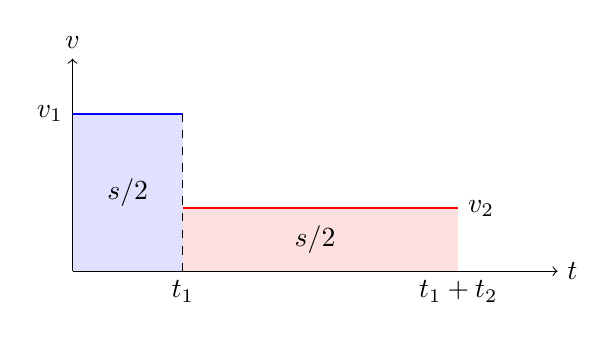
\begin{tikzpicture}[x=1.4cm,y=1cm]
\draw[->](0,0)--(4.4,0)node[right]{$t$};\draw[->](0,0)--(0,2.7)node[above]{$v$};
\fill[blue!12](0,0)rectangle(1,2);\fill[red!12](1,0)rectangle(3.5,.8);
\draw[blue,thick](0,2)--(1,2);\draw[red,thick](1,.8)--(3.5,.8);
\draw[dashed](1,0)--(1,2);\node[left]at(0,2){$v_1$};\node[right]at(3.5,.8){$v_2$};
\node at(.5,1){$s/2$};\node at(2.2,.4){$s/2$};\node[below]at(1,0){$t_1$};\node[below]at(3.5,0){$t_1+t_2$};\end{tikzpicture}}



\par\medskip\Needspace{4\baselineskip}\noindent\textbf{由剩余时间为正确定解的范围}\par\nobreak
图\ref{k1p1s}中每段时间与对应速度成反比，所以不能取速度的算术平均。存在条件可直接由第二段时间判断：$t_2=s/v-s/(2v_1)>0$，结合正的平均速度，得到 $0<v<2v_1$。代入 $v=v_1$有 $v_2=v_1$；当 $v\uparrow2v_1$时，$t_2\to0^+$而 $v_2\to\infty$，边界不能由有限速度实现。

若两段各自路程占总路程的比例为 $\lambda$、$1-\lambda$，相同推理给
\[\frac1{\bar v}=\frac{\lambda}{v_1}+\frac{1-\lambda}{v_2}.
\]
图\ref{k1p1q}的中点 $M$对应 $\lambda=1/2$。只有先明确是等路程而非等时间，这个调和平均关系才适用；两种平均式各自带有不同的权重。
\end{solution}

\begin{question}\begin{example}[一圈赛跑的平均量]\label{k1p2}
运动员从400m标准跑道的某点出发，40s后跑完一圈回到该点。求全程平均速度、平均速率，并判断能否据此确定跑到50m处的瞬时速度。\end{example}
\fig{k1p2q}{一圈赛跑的平均量：题设关系}{\begin{tikzpicture}\draw[world](0,0)ellipse(2.4 and 1);\fill(2.4,0)circle(1.5pt)node[right]{$A$};\draw[flow](0,1)--(.6,.97);\node at(0,0){$s=400\,\mathrm m$};\end{tikzpicture}}
\end{question}
\begin{solution}\textbf{分别计算起终点位移和沿跑道的路程}\par\nobreak
图\ref{k1p2q}中的起点与终点都是 $A$，故 $\Delta\bm r=\bm0$，全程平均速度为 $\bm0$；沿跑道的路程为400m，所以平均速率为 $400/40=\boxed{10\,\mathrm{m/s}}$。
\fig{k1p2s}{一圈赛跑的平均量：解答过程}{\begin{tikzpicture}\draw[axis](0,0)--(5,0)node[right]{$t$};\draw[axis](0,0)--(0,2.4)node[above]{$u$};\draw[world](0,1.2)--(4,1.2);\draw[blue](0,.4)--(4,2);\node[right]at(4,1.2){$10$};\node[below]at(4,0){$40$};\end{tikzpicture}}



\par\medskip\Needspace{4\baselineskip}\noindent\textbf{用两种可行速率过程检验信息是否充分}\par\nobreak
图\ref{k1p2s}画出两种总时间相同的速率变化示意：全程匀速和先慢后快可以有同样的图下面积。因此只有总路程、总用时不能确定50m处的瞬时速度。若额外假定全程匀速，才可说该处速率也为10m/s；这项假定不能从比赛成绩推出。平均速度为零也不意味着运动员全程静止。

在速率图中，400m约束的是 $\int_0^{40}u(t)\dd t=400$，而到50m的时刻应满足 $\int_0^{t_{50}}u(t)\dd t=50$。已知一个总积分，既不能唯一确定 $t_{50}$，也不能唯一确定该点的函数值 $u(t_{50})$。此外跑道在该位置的切线给速度方向，即使另知速率，也还要结合跑动方向确定速度矢量。\end{solution}

\begin{question}\begin{example}[速度图中的位移与路程]\label{k1p3}
质点沿直线运动：$0\le t\le1$s时 $v=3$m/s；$1\le t\le3$s时速度由3线性降至0；$3\le t\le6$s时速度由0线性降至$-3$m/s。求前3s及前6s的位移与路程。\end{example}
\fig{k1p3q}{速度图中的位移与路程：题设关系}{\begin{tikzpicture}\begin{scope}[x=.7cm,y=.4cm]\draw[axis](0,0)--(6.6,0)node[right]{$t/\mathrm s$};\draw[axis](0,-3.5)--(0,3.8)node[above]{$v/(\mathrm{m/s})$};\draw[world](0,3)--(1,3)--(3,0)--(6,-3);\foreach \x in {1,3,6}\node[below]at(\x,0){$\x$};\node[left]at(0,3){$3$};\node[left]at(0,-3){$-3$};\end{scope}\end{tikzpicture}}
\end{question}
\begin{solution}\textbf{按过零时刻划分正负面积}\par\nobreak
图\ref{k1p3q}在 $0$至3s内速度非负，矩形面积为 $3\times1=3$m，三角形面积为 $\tfrac12(3-1)\times3=3$m。因此 $\Delta x_3=s_3=\boxed{6\,\mathrm m}$。
\fig{k1p3s}{速度图中的位移与路程：解答过程}{\begin{tikzpicture}\begin{scope}[x=.7cm,y=.4cm]\draw[axis](0,0)--(6.6,0)node[right]{$t$};\fill[blue!15](0,0)--(0,3)--(1,3)--(3,0)--cycle;\fill[red!15](3,0)--(6,-3)--(6,0)--cycle;\draw[world](0,3)--(1,3)--(3,0)--(6,-3);\node at(1,1.1){$+6$};\node at(5,-1){$-4.5$};\end{scope}\end{tikzpicture}}


\par\medskip\Needspace{4\baselineskip}\noindent\textbf{反向阶段分别累计位移与路程}\par\nobreak
图\ref{k1p3s}中3至6s的阴影在时间轴下方，其面积数值为 $\tfrac12(6-3)\times3=4.5$m，表示反向位移。因此 $\boxed{\Delta x_6=6-4.5=1.5\,\mathrm m}$，而 $\boxed{s_6=6+4.5=10.5\,\mathrm m}$。在3s处速度过零并换号，正是累加路程时的分段点。结果满足 $s_6\ge|\Delta x_6|$。

\par\medskip\Needspace{4\baselineskip}\noindent\textbf{用分段积分核对图中面积}\par\nobreak
以秒为时间单位、米为长度单位，1至3s的速度函数是$v=3-\tfrac32(t-1)$，3至6s是$v=-(t-3)$。各段原函数及边界代入为
\begin{align*}
\Delta x_{0,1}&=\int_0^1 3\dd t=[3t]_0^1=3,\\
\Delta x_{1,3}&=\int_1^3\left[3-\frac32(t-1)\right]\dd t\\
&=\left[3(t-1)-\frac34(t-1)^2\right]_1^3
=(6-3)-0=3,\\
\Delta x_{3,6}&=\int_3^6[-(t-3)]\dd t
=\left[-\frac{(t-3)^2}{2}\right]_3^6
=-\frac92-0=-4.5.
\end{align*}
后一段速度为负，路程积分应改积$|v|=t-3$：
\[
s_{3,6}=\int_3^6(t-3)\dd t
=\left[\frac{(t-3)^2}{2}\right]_3^6=4.5.
\]
负速度表示坐标在减小，绝不是“走过负的路程”。把三段位移相加、各段路程相加，分别恢复图中算出的$1.5\,\mathrm m$与$10.5\,\mathrm m$。若再求前6s平均速度与平均速率，应分别除以同一个6s，得到0.25m/s和1.75m/s。\end{solution}

\begin{question}\begin{example}[由分段速度重建位置图]\label{k1p4}
取 $x(0)=0$，质点在三个连续且等长为 $T$ 的时间段内，速度依次为 $v_0,0,-v_0$，其中 $v_0>0$。写出位置函数并画出位置随时间变化的图。\end{example}
\fig{k1p4q}{由分段速度重建位置图：题设关系}{\begin{tikzpicture}
\draw[axis](0,0)--(5.5,0)node[right]{$t$};
\draw[axis](0,-1.3)--(0,1.5)node[above]{$v$};
\draw[world,blue](0,1)--(1.5,1) (1.5,0)--(3,0) (3,-1)--(4.5,-1);
\node[left]at(0,1){$v_0$};\node[left]at(0,-1){$-v_0$};
\foreach \x/\a in {1.5/T,3/2T,4.5/3T}\node[below]at(\x,0){$\a$};
\draw[guide](1.5,0)--(1.5,1) (3,0)--(3,-1) (4.5,0)--(4.5,-1);
\end{tikzpicture}}
\end{question}
\begin{solution}\textbf{逐段积分并继承前一段末位置}\par\nobreak
由图\ref{k1p4q}的三个速度平台逐段积分，连接点必须保持位置连续。第一段 $x(t)-x(0)=\int_0^t v_0\dd\tau=[v_0\tau]_0^t=v_0t$，故 $x(T)=v_0T$。第二段 $x(t)-x(T)=\int_T^t0\dd\tau=0$，故 $x(2T)=v_0T$。第三段 $x(t)-x(2T)=\int_{2T}^t(-v_0)\dd\tau=[-v_0\tau]_{2T}^t=-v_0(t-2T)$。三段合写为
\[x(t)=\begin{cases}v_0t,&0\le t\le T,\\v_0T,&T\le t\le2T,\\v_0(3T-t),&2T\le t\le3T.\end{cases}\]
\fig{k1p4s}{由分段速度重建位置图：解答过程}{\begin{tikzpicture}\draw[axis](0,0)--(5.2,0)node[right]{$t$};\draw[axis](0,0)--(0,2.3)node[above]{$x$};\draw[world](0,0)--(1.5,1.7)--(3,1.7)--(4.5,0);\draw[guide](1.5,1.7)--(1.5,0) (3,1.7)--(3,0);\node[left]at(0,1.7){$v_0T$};\node[below]at(1.5,0){$T$};\node[below]at(3,0){$2T$};\node[below]at(4.5,0){$3T$};\end{tikzpicture}}


\par\medskip\Needspace{4\baselineskip}\noindent\textbf{用位置图的斜率检查接续与总路程}\par\nobreak
图\ref{k1p4s}中第一段斜率为 $v_0$，第二段水平表示静止，第三段斜率为 $-v_0$，终点回到原点。速度在交界处发生理想化跳变，但位置没有竖直跳跃。全程位移为零、路程为 $2v_0T$；这与速度图的正、负面积相抵消相吻合。

第三段应从 $x(2T)=v_0T$出发写 $x=v_0T-v_0(t-2T)$，整理后才得到 $v_0(3T-t)$。若直接写成 $-v_0t$，相当于把第三段的时间原点和位置原点都错误地重置。两处连接点虽然连续，左右斜率却不相同，因此该理想位置函数在连接点不可导；应使用左右速度描述瞬间突变。\end{solution}

\begin{question}\begin{example}[延迟刹车的安全间距]\label{k1p5}
两辆相同汽车同向以速率 $v_0$ 行驶，初始车尾与后车车头之间的净间距为 $d$。前车以恒定减速度 $a$ 刹车，停车距离为 $s$；前车刚停下时，后车才以同一减速度刹车。两车停车后不倒退，求避免接触所需的 $d$。\end{example}
\fig{k1p5q}{延迟刹车的安全间距：题设关系}{\begin{tikzpicture}\draw[axis](0,0)--(6.7,0);\draw[world](.2,0)rectangle(1.7,.6) (4.1,0)rectangle(5.6,.6);\node at(.9,.3){后车};\node at(4.8,.3){前车};\draw[dim](1.7,-.6)--(4.1,-.6)node[midway,below]{$d$};\draw[flow](1.8,1)--(2.6,1)node[right]{$v_0$};\end{tikzpicture}}
\end{question}
\begin{solution}\textbf{分清前后两车各自的制动阶段}\par\nobreak
图\ref{k1p5q}采用净间距，故不必另计车长。前车在制动期间的加速度为$-a$，初速为$v_0$，先积分得到
\[
v_F(t)=v_0+\int_0^t(-a)\dd\tau
=v_0+[-a\tau]_0^t=v_0-at.
\]
令停车时刻$v_F(T)=0$，得到$T=v_0/a$。再积分速度求停车距离，
\begin{align*}
s&=\int_0^T(v_0-at)\dd t
=\left[v_0t-\frac{at^2}{2}\right]_0^T\\
&=v_0T-\frac{aT^2}{2}
=\frac{v_0T}{2}=\frac{v_0^2}{2a},
\end{align*}
其中用了$aT=v_0$。在前车制动阶段，后车比前车多走$v_0T-s=s$；后车随后制动又走$s$，而前车不再前进。
\fig{k1p5s}{延迟刹车的安全间距：解答过程}{\begin{tikzpicture}\draw[axis](0,0)--(5.5,0)node[right]{$t$};\draw[axis](0,0)--(0,2.5)node[above]{$v$};\fill[blue!12](0,2)--(2.3,2)--(4.6,0)--(2.3,0)--cycle;\draw[world](0,2)--(2.3,0)--(4.6,0);\draw[world,blue](0,2)--(2.3,2)--(4.6,0);\node[below]at(2.3,0){$T$};\node[below]at(4.6,0){$2T$};\node at(1.5,1){$s$};\node at(3,.6){$s$};\end{tikzpicture}}



\par\medskip\Needspace{4\baselineskip}\noindent\textbf{从相对位移面积找全程最小间距}\par\nobreak
图\ref{k1p5s}的速度差始终非负，两个三角形面积之和为 $2s$，因此间距单调减小，最小值出现在两车都停住时：$d_{\min}=d-2s$。允许刚好接触的临界值为 $\boxed{d=2s}$；若要求严格不接触，应取 $\boxed{d>2s}$。只检查前车停住的一刻会漏掉后车自己的停车距离。

把初始间距减去累计接近量，可将全程净间距写为
\[D(t)=\begin{cases}d-\tfrac12at^2,&0\le t\le T,\\
d-s-v_0(t-T)+\tfrac12a(t-T)^2,&T\le t\le2T.
\end{cases}\]
两段分别满足 $\dot D=-at\le0$和 $\dot D=-v_0+a(t-T)\le0$，连接处同为 $d-s$，终点为 $d-2s$。这不仅算出了最终差值，也证明途中没有更小间距，因而安全条件具有全程意义。

% thirty-k1-braking

\par\medskip\Needspace{4\baselineskip}\noindent\textbf{推广到任意反应延迟并检查停车边界}\par\nobreak
还可推广到一般反应延迟 $\tau\ge0$，与本题制动时间 $T=v_0/a$区分。令
$f(t)=\max(v_0-at,0)$为前车速度，则后车在 $0\le t<\tau$速度为 $v_0$，在 $t\ge\tau$速度为 $f(t-\tau)$。由于 $f$单调不增，后车速度在全程都不小于前车，净间距因此始终不增。

将图\ref{k1p5s}中的后车速度曲线水平平移 $\tau$，后车总路程为 $v_0\tau+s$，前车总路程为 $s$。无论 $\tau<T$还是 $\tau\ge T$，总接近量都为
\[(v_0\tau+s)-s=v_0\tau.\]
所以不出现负间距的条件为 $d\ge v_0\tau$，严格不接触则为 $d>v_0\tau$。代回本题 $\tau=T$，得到 $v_0T=2s$，与分段积分完全一致。推广时必须把已停车车辆的速度置零；若继续沿直线把它算成负速度，便会虚构倒退并夸大危险。
\end{solution}

\begin{question}\begin{example}[定时发车与途中相遇]\label{k1p6}
$A,B$两站相距60km。自 $t=0$ 起，$A$站每隔10min发出一辆速度为60km/h的汽车驶向 $B$。$B$站一车也以60km/h驶向 $A$，并选择在 $A$站某次发车的同时出发。只计两站之间的相遇，不计在站内相遇。求最多遇车数和达到此数量的最早出发时刻。\end{example}
\fig{k1p6q}{定时发车与途中相遇：题设关系}{\begin{tikzpicture}\draw[axis](0,0)--(6.2,0)node[right]{$x$};\node[below]at(0,0){$A$};\node[below]at(5.5,0){$B$};\draw[flow](.5,.6)--(2,.6)node[above]{$60$};\draw[flow](5,.6)--(3.5,.6)node[above]{$60\ \mathrm{km/h}$};\draw[dim](0,-.6)--(5.5,-.6)node[midway,below]{$60\,\mathrm{km}$};\end{tikzpicture}}
\end{question}
\begin{solution}\textbf{按发车序号写出各车的运动时段}\par\nobreak
图\ref{k1p6q}两站单程时间为 $T=60\,\mathrm{min}$，发车间隔为 $\tau=10\,\mathrm{min}$。从 $A$出发的第 $k$辆车在 $k\tau$发车，$k=0,1,\ldots$；令 $B$车在 $t_b=m\tau$出发，$m$为非负整数。将路程与速度均换成千米、分钟后，位置方程为
\[x_A=u(t-k\tau),\qquad x_B=uT-u(t-t_b),
\qquad u=1\,\mathrm{km/min}.\]
相遇要求$x_A=x_B$，约去$u>0$得到$t-k\tau=T-t+t_b$，所以$t=(T+t_b+k\tau)/2$。它还必须发生在两车各自离站后、到站前。分别列出有效时间区间，并代入这个相遇时刻：
\begin{align*}
k\tau<t<k\tau+T
&\quad\Longrightarrow\quad t_b-T<k\tau<t_b+T,\\
t_b<t<t_b+T
&\quad\Longrightarrow\quad t_b-T<k\tau<t_b+T.
\end{align*}
两车的限制恰好给出同一组严格不等式：
\[t_b-T<k\tau<t_b+T,\qquad k\ge0.\]
这里不能取等号，因为等号对应站内相遇。

用 $T=6\tau$、$t_b=m\tau$化简，允许的整数满足
\[m-6<k<m+6,\quad k\ge0,
\qquad k=\max(0,m-5),\ldots,m+5.\]
其数量为 $m+5-\max(0,m-5)+1$：$m<5$时为 $m+6$，$m\ge5$时为11。因此最多遇到 $\boxed{11\text{辆}}$，首次达到这一数量的出发时刻为 $\boxed{50\,\mathrm{min}}$。
\fig{k1p6s}{位置时间图中的红色交点计入，站点端点排除}{\begin{tikzpicture}[x=1.25cm,y=1.5cm]
\draw[axis](0,0)--(4.5,0)node[right]{$t/(30\,\mathrm{min})$};\draw[axis](0,0)--(0,2.5)node[above]{$x/(30\,\mathrm{km})$};
\begin{scope}\clip(0,0)rectangle(4.1,2);
\foreach \k in {0,...,11}\draw[gray]({\k/3},0)--({\k/3+2},2);
\draw[blue,very thick](1.666667,2)--(3.666667,0);
\foreach \k in {0,...,10}\fill[red]({(11+\k)/6},{(11-\k)/6})circle(1pt);
\end{scope}
\draw[guide](0,2)--(4.1,2);\node[left]at(0,2){$B$};\node[below left]at(0,0){$A$};
\draw[fill=white](3.666667,0)circle(1.4pt);\node[above,blue]at(1.666667,2){出发};\node[below]at(3.666667,0){到站};
\end{tikzpicture}}



\par\medskip\Needspace{4\baselineskip}\noindent\textbf{剔除站点相见并核对计数边界}\par\nobreak
图\ref{k1p6s}特取 $t_b=50\,\mathrm{min}$。此时 $k=0,1,\ldots,10$，相遇时刻为 $t_k=55+5k$分钟，均严格落在 $(50,110)$内；相邻相遇间隔是5分钟。第11号车于110分钟在 $A$发车，与 $B$车恰在站点相见，对应图中的空心端点，不计入红点数量。

整数范围与交点图共同检验了最大数目及最早出发时刻。
\end{solution}

\begin{question}\begin{example}[两根平移直杆的交点]\label{k1p7}
两根足够长直杆 $A,B$ 与水平线分别成 $30^\circ,60^\circ$，$A$从左下向右上倾斜，$B$从左上向右下倾斜。$A$以速率 $v_A$ 向左平移，$B$以速率 $v_B$ 向右平移。求交点 $C$ 的速度，并分别讨论其中一杆静止的情形。\end{example}
\fig{k1p7q}{两根平移直杆的交点：题设关系}{\begin{tikzpicture}\draw[world](-2,-.9)--(2.6,1.76)node[right]{$A$};\draw[world](-.9,1.809)--(.8,-1.136)node[right]{$B$};\fill(0,.25)circle(1.4pt)node[above left]{$C$};\draw[guide](-2,-.9)--(3,-.9);\node at(-.9,-.65){$30^\circ$};\draw[guide](.66,-.9)--(-.7,-.9);\node at(.12,-.57){$60^\circ$};\draw[flow](-1,-1.5)--(-2,-1.5)node[left]{$v_A$};\draw[flow](1,-1.5)--(2,-1.5)node[right]{$v_B$};\end{tikzpicture}}
\end{question}
\begin{solution}\textbf{用两条随时间平移的直线确定交点}\par\nobreak
取图\ref{k1p7q}中初始交点为原点，向右、向上为正。为保留一般倾角的结果，先记 $p=\tan\theta$、$q=\tan\varphi$，其中 $\theta,\varphi$为两杆分别与水平线所成的锐角。杆 $A$向左、杆 $B$向右平移，交点同时满足
\[y=p(x+v_At),\qquad y=-q(x-v_Bt).\]
两式均对同一时间求导，再消去 $v_y$：
\[v_y=p(v_x+v_A)=q(v_B-v_x),\]
\[
(p+q)v_x=qv_B-pv_A,\qquad
v_x=\frac{qv_B-pv_A}{p+q}.
\]
把此水平分量代回$v_y=p(v_x+v_A)$，再通分合并：
\[
v_y=p\left(\frac{qv_B-pv_A}{p+q}+v_A\right)
=\frac{p(qv_B-pv_A+pv_A+qv_A)}{p+q}
=\frac{pq(v_A+v_B)}{p+q}.
\]
本题代入 $p=1/\sqrt3$、$q=\sqrt3$，得到
\[\boxed{v_x=\frac{3v_B-v_A}{4}},\qquad
\boxed{v_y=\frac{\sqrt3(v_A+v_B)}4}.\]
\fig{k1p7s}{两根平移直杆的交点：解答过程}{\begin{tikzpicture}\draw[axis](0,0)--(3.5,0)node[right]{$x$};\draw[axis](0,0)--(0,2.5)node[above]{$y$};\draw[flow,blue](0,0)--(2,1.7)node[above right]{$\bm v_C$};\draw[guide](2,0)--(2,1.7)--(0,1.7);\node[below]at(1,0){$v_x$};\node[left]at(0,1){$v_y$};\end{tikzpicture}}



\par\medskip\Needspace{4\baselineskip}\noindent\textbf{合成分量并区分交点与杆上物质点}\par\nobreak
图\ref{k1p7s}中的方向由分量的符号决定。两分量平方相加时，交叉项恰好抵消：
\[|\bm v_C|^2=\frac{(3v_B-v_A)^2+3(v_A+v_B)^2}{16}
 =\frac{v_A^2+3v_B^2}{4}.\]
所以速率为 $\tfrac12\sqrt{v_A^2+3v_B^2}$。题设另问的一杆静止情形，直接在同一结果中代入：
\begin{align*}
v_A=0:\quad &(v_x,v_y)=\left(\frac{3v_B}{4},\frac{\sqrt3v_B}{4}\right),
 &|\bm v_C|=\frac{\sqrt3}{2}v_B;\\
v_B=0:\quad &(v_x,v_y)=\left(-\frac{v_A}{4},\frac{\sqrt3v_A}{4}\right),
 &|\bm v_C|=\frac{v_A}{2}.
\end{align*}
前者沿静止的 $A$杆向右上运动，后者沿静止的 $B$杆向左上运动；这也分别检查了 $30^\circ$与 $120^\circ$的速度方向。

两杆都运动时，$v_y>0$，但 $v_x$可以改变符号：$v_A<3v_B$时向右上，$v_A>3v_B$时向左上；$v_A=3v_B$时交点恰沿竖直方向，速率为 $\sqrt3v_B$。因此交点的方向不必沿任一根杆。

最后核对物质身份。相对 $A$杆的速度为 $\bm v_C-(-v_A,0)$，相对 $B$杆的速度为 $\bm v_C-(v_B,0)$，它们的斜率分别为 $p$和 $-q$，均沿对应杆。交点可以沿两杆材料滑动，不能再附加“交点与某一杆上固定物质点同速”的条件。
\end{solution}

\begin{question}\begin{example}[速度随高度变化的爬行]\label{k1p8}
蜗牛从电杆底部向上爬，速度与高度关系为 $v(h)=lv_0/(l+h)$，其中 $l=20$cm，$v_0=2$cm/s。求爬高20cm的时间，并用图像说明积分的意义。\end{example}
\fig{k1p8q}{速度随高度变化的爬行：题设关系}{\begin{tikzpicture}\draw[world](0,0)--(0,3.2);\draw[axis](.8,0)--(.8,3.2)node[above]{$h$};\fill(0,1.4)circle(2pt)node[left]{蜗牛};\draw[flow](0,1.6)--(0,2.3)node[left]{$v(h)$};\node[right]at(.8,2.7){$20\,\mathrm{cm}$};\end{tikzpicture}}
\end{question}
\begin{solution}\textbf{按高度微元累积倒速度}\par\nobreak
图\ref{k1p8q}中 $h$ 单调增加，微小高度 $\dd h$ 的用时为 $\dd t=(l+h)\dd h/(lv_0)$，所以
\[t=\int_0^l\frac{l+h}{lv_0}\dd h
 =\frac1{lv_0}\left[lh+\frac{h^2}{2}\right]_0^l
 =\frac{l^2+l^2/2}{lv_0}=\boxed{15\,\mathrm s}.\]
\fig{k1p8s}{速度随高度变化的爬行：解答过程}{\begin{tikzpicture}\draw[axis](0,0)--(5,0)node[right]{$h/\mathrm{cm}$};\draw[axis](0,0)--(0,2.7)node[above]{$1/v$};\fill[blue!12](0,0)--(0,1)--(4,2)--(4,0)--cycle;\draw[world](0,1)--(4,2);\node[left]at(0,1){$0.5$};\node[left]at(0,2){$1$};\node[below]at(4,0){$20$};\end{tikzpicture}}



\par\medskip\Needspace{4\baselineskip}\noindent\textbf{用梯形面积和速度上下界核验}\par\nobreak
图\ref{k1p8s}将纵轴取为 $1/v$，它随 $h$ 线性增加。梯形两条平行边分别为 $1/v_0=0.5$和 $2/v_0=1$，单位为s/cm，底长20cm，面积为 $20(0.5+1)/2=15$s。速度从2降至1cm/s，所得用时在10s与20s之间，符合快慢界限；若误取 $v$--$h$ 面积，量纲便不是时间。

若积分上限改为任意爬高$H$，同样的原函数给出
\[
t(H)=\frac1{lv_0}\left[lh+\frac{h^2}{2}\right]_0^H
=\frac{lH+H^2/2}{lv_0}
=\frac H{v_0}+\frac{H^2}{2lv_0}.
\]
固定$l,v_0$，对$H$逐项求导有
\[
\frac{\dd t}{\dd H}=\frac1{v_0}+\frac{2H}{2lv_0}
=\frac{l+H}{lv_0}=\frac1{v(H)},
\]
代回即恢复题设。$H\ll l$时第二项相对较小，才可近似按初速匀速计算；本题$H=l$，该项占总时间三分之一，不能忽略。这里积分的对象是每小段的用时，而不是将首末速度简单平均。

% thirty-k1-climbtime

\par\medskip\Needspace{4\baselineskip}\noindent\textbf{反求位置随时间的变化并核对速度}\par\nobreak
还能将积分关系反解为随时间变化的位置，以检验模型的全过程。由
\[v_0t=h+\frac{h^2}{2l}\]
两边乘 $2l$并配方，得到 $(h+l)^2=l^2+2lv_0t$。因 $h\ge0$，必须取正平方根：
\[h(t)=l\left(\sqrt{1+\frac{2v_0t}{l}}-1\right).\]
第一次求导保留根式与内层两因子，$\dot h=l\cdot\tfrac12(1+2v_0t/l)^{-1/2}\cdot(2v_0/l)=v_0/\sqrt{1+2v_0t/l}=lv_0/(l+h)$，恰好恢复题设；第二次同样先写 $\ddot h=v_0(-\tfrac12)(1+2v_0t/l)^{-3/2}(2v_0/l)$，化简为
\[\ddot h=-\frac{v_0^2}{l}
 \left(1+\frac{2v_0t}{l}\right)^{-3/2}<0.\]
所以蜗牛始终向上而逐渐减速。令 $h=l$，则平方根等于2，给出 $t=3l/(2v_0)=15\,\mathrm s$。
\fig{k1p8history}{位置曲线的斜率递减，但高度始终增加}{\begin{tikzpicture}
\draw[axis](0,0)--(4.6,0)node[right]{$v_0t/l$};
\draw[axis](0,0)--(0,2.4)node[above]{$h/l$};
\draw[world,blue]plot[domain=0:2,samples=60]({2*\x},{1.8*(sqrt(1+2*\x)-1)});
\draw[guide](3,0)--(3,1.8)--(0,1.8);
\node[below]at(3,0){$3/2$};\node[left]at(0,1.8){$1$};
\end{tikzpicture}}
图\ref{k1p8history}中的无量纲曲线不依赖厘米或米的选择。两个参数 $l,v_0$只确定高度尺度 $l$与时间尺度 $l/v_0$；计算前统一长度单位，便能同时检验公式量纲与数值代入。
\end{solution}
